%!TEX TS-program = xelatex
\documentclass[a4paper, 12pt]{article}
\usepackage{barinovxesimple}
\usepackage[version=4]{mhchem}
\geometry{top=25mm}
\geometry{bottom=35mm}
\geometry{left=35mm}
\geometry{right=20mm}
\setlist{labelindent=\parindent,leftmargin=*}
\begin{document}
\thispagestyle{empty}
\begin{center}
    \textit{Федеральное государственное автономное образовательное\\ учреждение высшего образования }

    \vspace{0.5ex}

        \textbf{«Московский физико-технический институт\\ (национальный исследовательский университет)»}
\end{center}

\vspace{10ex}

\begin{center}
    \vspace{13ex}

    \so{\textbf{Лабораторная работа №-.-.-}}

    \vspace{1ex}

    по курсу общей физики

    на тему:

    \textbf{\textit{<<>>}}

    \vspace{30ex}

    \begin{flushright}
        \noindent
        \textit{Работу выполнил:}\\  
        \textit{Баринов Леонид \\(группа Б02-827)}
    \end{flushright}
    \vfill
    Долгопрудный \\2019
\newpage
\setcounter{page}{1}
\fancyhead[R]{\nouppercase{\leftmark}}	
\end{center}

\section{Цель работы}
Исследовать энергетический спектр $\beta$-частиц при распаде ядер
$ ^{137}$Cs и определить их максимальную энергию.

\section{Суть исследуемого явления}
$\beta$-распад - самопроизвольное превращение ядер, при котором их
массовое число не изменяется, а заряд увеличивается или уменьшается на
единицу.


\section{Теория явления}
В данной работе будет рассмотрен электронный распад:
\[
    \ce{^{A}_{Z}X} \rightarrow \ce{^{A}_{Z+1} X} + e ^{-} + \tilde
    \nu,
\]

Доля энергии, передаваемая ядру, крайне мала по сравнению с энергией
уносимой электроном и антинейтрино, поэтому можно считать что эти
частицы делят между собой всю освобождающуюся энергию.

Запишем закон сохранения энергии:
\begin{equation}
    E_e - T - ck = 0,
    \label{eq:1}
\end{equation}
где $E_e$ --- максимальная энергия электрона, $T$ --- кинетическая
энергия электрона, $ck$ --- энергия
антинейтрино с импульсом $k$. 
\begin{equation}
    T = c \sqrt{p^2 + m^2c^2} - mc^2
    \label{eq:2}
\end{equation}

Вероятность $d \omega$ того, что при распаде электрон вылетит с
импульсом $d^3 \vec{p}$, а антинейтрино с импульсом в интервале $d^3
\vec{k}$ пропорциональна произведению этих дифференциалов.

\begin{equation}
    d \omega = D \delta (E_e - E -ck) d^3 \vec{p} d^3 \vec{k} = D
    \delta (E_e - E - ck)p^2 dp k^2 dk d\Omega_e d\Omega _{\tilde \nu}
    \label{eq:3}
\end{equation}
где $D$ --- некоторый коэффициент пропорциональности, $d\Omega_e$,
$d\Omega _{\tilde \nu}$ --- элементы телесных углов направлений вылета
электрона и нейтрино.

Вероятность $d\omega$ непосредственно связана с
$\beta$-спектром, поскольку для очень большого числа $N_0$ распадов
$dN$ распадов с вылетом электрона и антинейтрино с импульсом
соответственно от $\vec{p}$ до $\vec{p} + d \vec{p}$ и от $\vec{k}$ до
$\vec{k} + d \vec{k}$ определяется соотношением
\begin{equation}
    dN = N_0 d \omega
    \label{eq:4}
\end{equation}

Проинтегрируем уравнение \eqref{eq:3} по телесным углам и по $k$
\begin{equation}
    d N = \frac{16 \pi^2 N_0}{c^2} D p^2 (E_e - T)^2 dp
    \label{eq:5}
\end{equation}

Перейдем от $dp$ к $dT$:
\begin{equation}
    dT = \frac{c^2 p}{T + mc^2}dp
    \label{eq:6}
\end{equation}


\begin{equation}
    \begin{aligned}
        \frac{dN}{dT} &= N_0 B cp (T + mc^2) (E_e - T)^2 = 
        \\ &= N_0 B \sqrt{T (T + 2mc^2)} (E_e - T)^2 (T + mc^2) 
    \end{aligned}
    \label{eq:7}
\end{equation}


\noindent где $B = (16 \pi^2 / c^4)D$. В нерелятивистском приближении, которое и
имеет место в нашей случае, выражение \eqref{eq:7} упрощается:
\begin{equation}
    \frac{dN}{dT} \approx \sqrt{T} (E_e - T)^2
    \label{eq:8}
\end{equation}

\begin{wrapfigure}{l}{0.33\linewidth}
    \vspace{-3em}
    \includegraphics[width=\linewidth]{1}
    \caption{Форма спектра $\beta$-частиц при разрешенных переходах}
    \label{fig:1}
\end{wrapfigure}

Выражение \eqref{eq:8} приводит к спектру, имеющему вид широкого
колокола \ffig{fig:1}. Дочерние ядра, возникающие в результате
$\beta$-распада, нередко оказываются возбужденными. Возбужденные ядра
отдают свою энергию либо излучая $\gamma$-квант, либо передавая
избыток энергии одного из электронов с внутренних оболочек атома.
Излученные в таком процессе электроны имеют строго определенную
энергию и называются \emph{конверсионными}.

На \fig{fig:1} видна монохроматическая линия, вызванная электронами
конверсии.  Ширина этой линии в нашем случае является чисто
аппаратурной --- по ней можно оценить разрешающую силу спектрометра.


\section{Эксперимент}
\subsection{Экспериментальная установка}
Энергию $\beta$-частиц определяют с помощью $\beta$-спектрометров. В
работе используется магнитный спектрометр с <<короткой линзой>>.
Электрона, испускаемые радиоактивным источником \ffig{fig:2}, попадают
в магнитное поле катушки, ось которой параллельна оси $OZ$.


\begin{figure}[H]
    \includegraphics[width=0.7\linewidth]{2} 
    \caption{Схема $\beta$-спектрометра с короткой магнитной линзой}
    \label{fig:2}
\end{figure}

Траектории электронов в магнитном поле представляют собой
схематически показанные на рисунке сложные спирали, сходящиеся за
катушкой в фокусе, расположенном на оси $OZ$. Силовые линии магнитного
поля изображены на $\fig{fig:2}$ тонкими линиями. В фокусе установлен
детектор электронов --- газоразрядный торцевой счетчик с тонким
входным окном, прозрачным для электронов с энергией больше $40\:
\text{кэВ}$, либо сцинтилляционный счетчик.

Для заряженных частиц тонкая катушка эквивалентна линзе. Ее фокусное
расстояние $f$ зависит от импульса электронов $p_e$ и от индукции
магнитного поля линзы (т.е. от силы тока $I$, протекающего через
катушку) следующим образом:
\begin{equation}
    \frac{1}{f} \propto \frac{I^2}{p_e^2}
    \label{eq:9}
\end{equation}

Импульс сфокусированных электронов пропорционален величине тока $I$:
\begin{equation}
    p_e = k I
    \label{eq:10}
\end{equation}

Рассмотрим связь между числом частиц, регистрируемых установкой, и
функцией $W (p_e) = dW / dp_e$, определяемой формулой \eqref{eq:8} 
\begin{equation}
    N (p_e) \simeq W (p_e) \Delta p_e
    \label{eq:11}
\end{equation}
где $\Delta p_e$ --- разрешающая способность спектрометра. Формула
\eqref{eq:9} показывает, что при заданном токе фокусное расстояние
магнитной линзы зависит от импульса частиц. Мимо счетчика проходят
частицы, для которых фокусное расстояние линзы слишком сильно
отличается от нужного, т.е. при недопустимо больших $\Delta f$.

Дифференцируем формулу \eqref{eq:9} при постоянном токе:
\begin{equation}
    \Delta p_e = \frac{1}{2} \frac{\Delta f}{f}p_e
    \label{eq:12}
\end{equation}

Таким образом, ширина интервала $\Delta p_e$, регистрируемого
спектрометром, пропорциональна величине импульса. Подставив
\eqref{eq:12} в \eqref{eq:11} и замечая, что отношение $\Delta f/ 2f$
определяется геометрией установки и потому постоянно, получим
окончательно:
\begin{equation}
    N (p_e) = C W (p_e) p_e,
    \label{eq:13}
\end{equation}
где $C$ --- некоторая константа.

Блок-схема установки для изучения $\beta$-спектров изображена на
\fig{fig:3}.


\begin{figure}[H]
    \includegraphics[width=0.8\linewidth]{3} 
    \caption{Блок-схема установки для изучения $\beta$-спектра}
    \label{fig:3}
\end{figure}

\section{Результаты эксперимента}

\renewcommand{\arraystretch}{1.3}
\begin{longtable}{|c|c|c|c|c|c|}
\hline 
$I,\: \text{A}$ & $N,\: \text{1/с}$ & $N - N_\text{ф},\: \text{1/c}$ &
$p,\: \text{кэВ/с}$ & $T,\: \text{кэВ}$ & \begin{tabular}{c}  
    $\sqrt{N(p)}/p ^{3/2} \cdot 10 ^{-6}$, \\ 
    $\text{c}^{-1/2}/ (\text{кэВ})^{3/2}$ 
\end{tabular} \\ \hline 
	\endfirsthead
        \hline 
$I,\: \text{A}$ & $N,\: \text{1/с}$ & $N - N_\text{ф},\: \text{1/c}$ &
$p,\: \text{кэВ/с}$ & $T,\: \text{кэВ}$ & \begin{tabular}{c}  
    $\sqrt{N(p)}/p ^{3/2} \cdot 10 ^{-6}$, \\ 
    $\text{c}^{-1/2}/ (\text{кэВ})^{3/2}$ 
\end{tabular} \\ \hline 
	\endhead
	\hline
	\endfoot

	\endlastfoot
0,00 & 0,650 & -0,025 & 0,00     & 0,00   & 0,000    \\ \hline
0,20 & 0,850 & 0,175  & 49,40    & 2,40   & 1204,673 \\ \hline
0,40 & 0,875 & 0,200  & 98,70    & 9,50   & 455,366  \\ \hline
0,60 & 0,575 & -0,100 & 148,10   & 21,00  & 0,000    \\ \hline
0,80 & 1,187 & 0,512  & 197,50   & 36,80  & 257,823  \\ \hline
1,00 & 1,200 & 0,525  & 246,90   & 56,50  & 186,723  \\ \hline
1,20 & 1,649 & 0,974  & 296,20   & 79,70  & 193,594  \\ \hline
1,40 & 1,962 & 1,287  & 345,60   & 105,90 & 176,546  \\ \hline
1,60 & 2,474 & 1,799  & 395,00   & 134,90 & 170,862  \\ \hline
1,80 & 2,774 & 2,099  & 444,40   & 166,20 & 154,666  \\ \hline
2,00 & 3,074 & 2,399  & 493,70   & 199,60 & 141,176  \\ \hline
2,20 & 2,649 & 1,974  & 543,10   & 234,70 & 111,005  \\ \hline
2,40 & 3,361 & 2,686  & 592,50   & 271,40 & 113,647  \\ \hline
2,50 & 3,036 & 2,361  & 617,20   & 290,30 & 100,224  \\ \hline
2,60 & 3,374 & 2,699  & 641,90   & 309,40 & 101,023  \\ \hline
2,80 & 2,861 & 2,186  & 691,20   & 348,60 & 81,364   \\ \hline
2,90 & 2,736 & 2,061  & 715,90   & 368,60 & 74,954   \\ \hline
3,00 & 2,074 & 1,399  & 740,60   & 388,80 & 58,690   \\ \hline
3,15 & 1,937 & 1,262  & 777,60   & 419,50 & 51,799   \\ \hline
3,20 & 1,812 & 1,137  & 790,00   & 429,80 & 48,020   \\ \hline
3,30 & 1,637 & 0,962  & 814,70   & 450,70 & 42,178   \\ \hline
3,40 & 1,087 & 0,412  & 839,30   & 471,70 & 26,398   \\ \hline
3,50 & 1,137 & 0,462  & 864,00   & 492,80 & 26,764   \\ \hline
3,60 & 1,175 & 0,500  & 888,70   & 514,20 & 26,677   \\ \hline
3,70 & 0,800 & 0,125  & 913,40   & 535,60 & 12,791   \\ \hline
3,80 & 1,562 & 0,887  & 938,10   & 557,20 & 32,777   \\ \hline
3,90 & 2,674 & 1,999  & 962,80   & 579,00 & 47,328   \\ \hline
4,00 & 2,786 & 2,111  & 987,50   & 600,80 & 46,828   \\ \hline
4,05 & 3,124 & 2,449  & 999,80   & 611,80 & 49,499   \\ \hline
4,08 & 3,336 & 2,661  & 1007,20  & 618,40 & 51,033   \\ \hline
4,10 & 3,948 & 3,273  & 1012,20  & 622,80 & 56,187   \\ \hline
4,15 & 3,849 & 3,174  & 1024,50  & 633,90 & 54,325   \\ \hline
4,20 & 3,336 & 2,661  & 1036,80  & 644,90 & 48,862   \\ \hline
4,25 & 3,186 & 2,511  & 1049,20  & 656,00 & 46,630   \\ \hline
4,30 & 3,111 & 2,436  & 1061,50  & 667,10 & 45,130   \\ \hline
4,35 & 2,586 & 1,911  & 1073,90  & 678,20 & 39,288   \\ \hline
4,40 & 1,837 & 1,162  & 1086,20  & 689,40 & 30,109   \\ \hline
4,50 & 0,962 & 0,287  & 1110,90  & 711,80 & 14,472   \\ \hline
4,55 & 0,437 & -0,238 & 1123,20  & 723,00 & 0,000    \\ \hline
4,60 & 0,475 & -0,200 & 1135,60  & 734,30 & 0,000    \\ \hline
4,70 & 0,462 & -0,213 & 1160,30  & 756,80 & 0,000    \\ \hline

\caption{1, 2 колонки - зависимость числа частиц, регистрируемых счетчиком в одну
    секунду $N$, от тока магнитной линзы $I$. 3 колонка - поправка на
    фон. 4, 5 колонки -  вычисленные
значения импульса $p$ и энергии электронов $T$. 5 колонка - расчет,
необходимый для построения графика Ферми-Кюри }
    
\end{longtable}



\begin{figure}[H]
    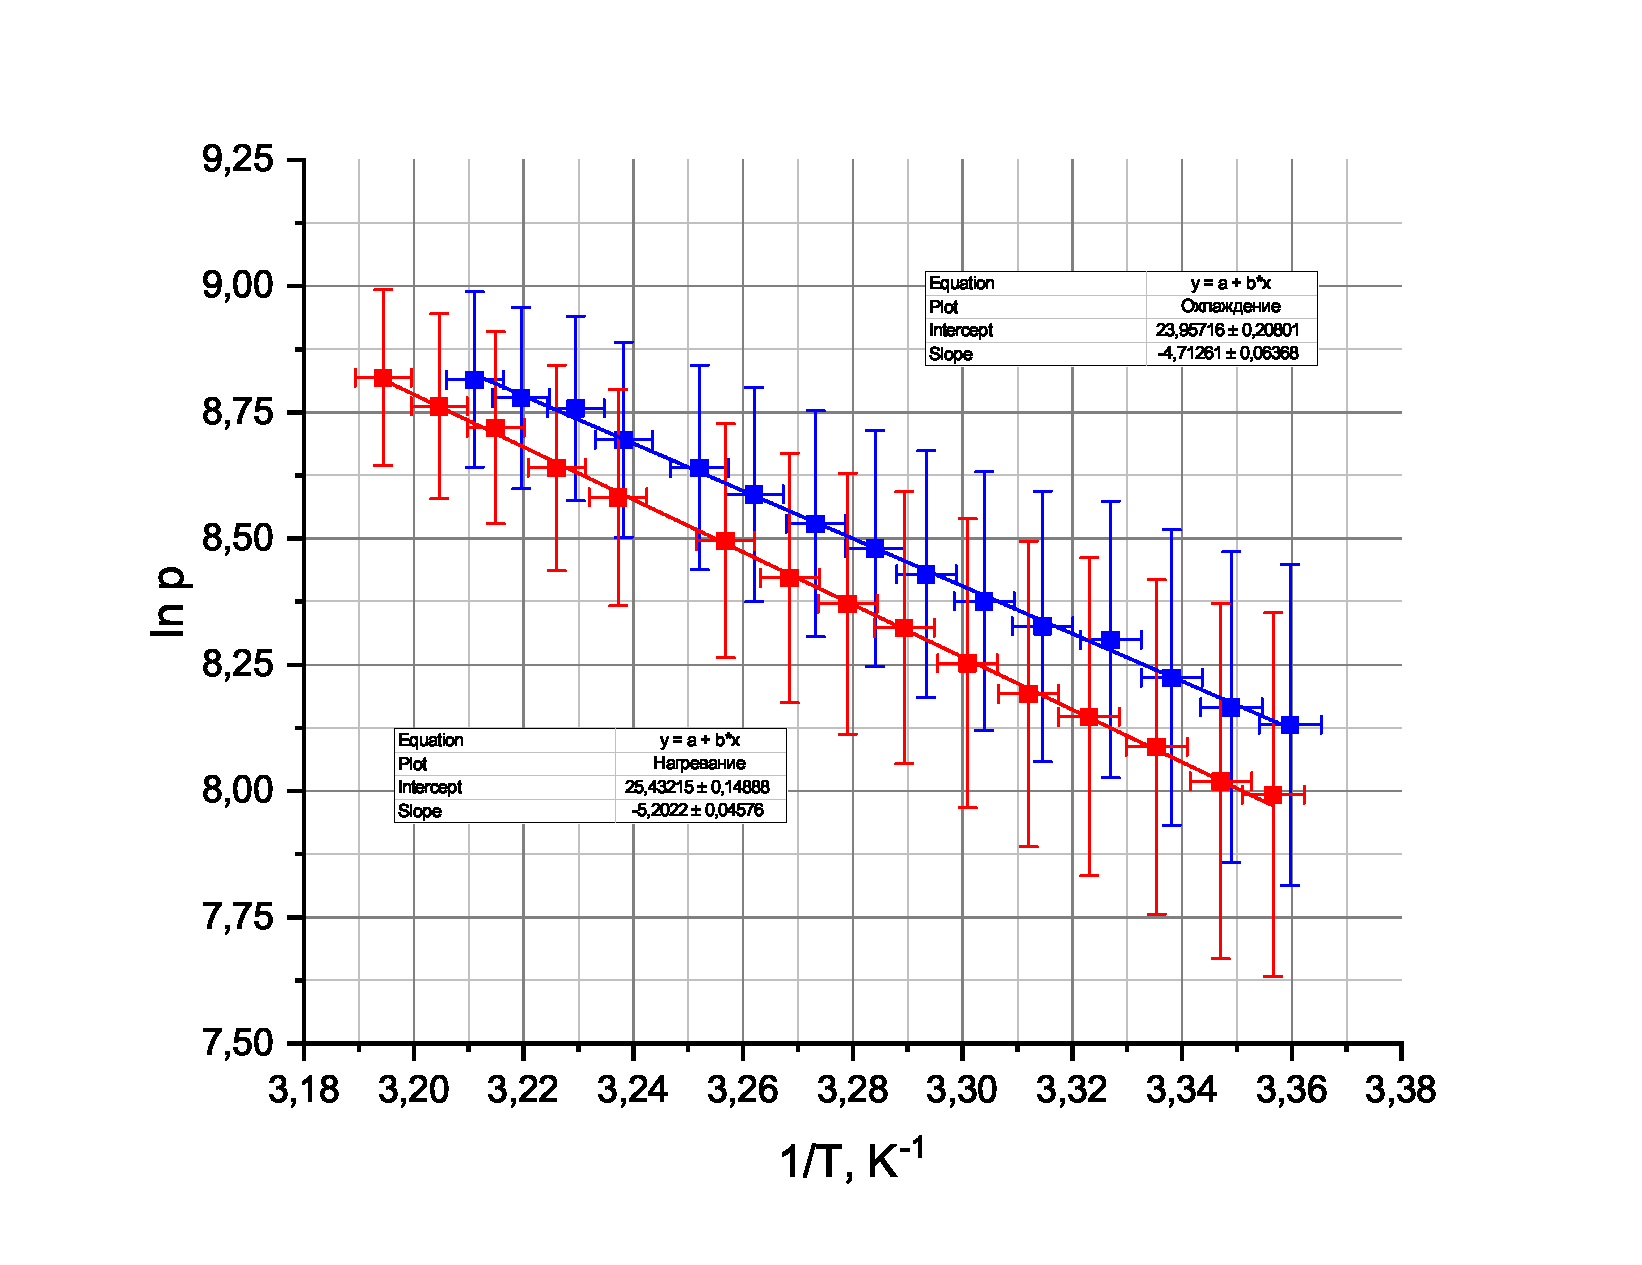
\includegraphics[width=\linewidth]{4} 
    \caption{График зависимости числа частиц в секунду $N$ от тока
    магнитной линзы $I$}
    \label{fig:4}
\end{figure}


\begin{figure}[H]
    \includegraphics[width=\linewidth]{5} 
    \caption{График Ферми-Кюри}
    \label{fig:5}
\end{figure}

\section{Анализ результатов}

По графику на \fig{fig:4} виден характер спектра:
непрерывная часть обеспечивается за счет рождения двух частиц, которые
делят между собой всю освобождающуюся энергию,
дискретный пик --- рождения конверсионных электронов. Непрерывность
спектра доказывает существование антинейтрино и его рождение в
процессе $\beta$-распада. Было выяснено существование
конверсионных электронов --- частиц, испускаемых в результате перехода
ядра на более низкий энергетический уровень, их энергетический спектр
уже является дискретным, так как их энергия строго привязана к энергии
электронных уровней в атоме.

Экстраполируя график Ферми-Кюри \ffig{fig:5} в районе убывания к оси абсцисс, определим
значение 
\[
    T _{\text{max}} = (556 \pm 23)\: \text{кэВ} 
\]








\section{Выводы}
В работе был изучен спектр $\beta$-распада $^{137}$Cs \ffig{fig:4}.
Экспериментальным путем найден конверсионный пик и оценено максимальное
значение энергии электрона в этом распаде 
\[
    T_\text{max} = (556 \pm 23)\: \text{кэВ} 
\]

Полученное значение в пределах погрешности достаточно точно совпадает
с теоретическим
значением:
\[
    T \simeq 512\: \text{кэВ}
\]

Неточность связана с временем детектирования частиц и с возможностью
разрешения 
установки.


























\end{document}
